\documentclass{article} \usepackage{amsmath} \usepackage{amssymb} \usepackage{amsthm} \usepackage[margin=0.2in]{geometry} \usepackage{hyperref} \usepackage{physics} \usepackage{tikz} \usepackage{mathtools} \mathtoolsset{showonlyrefs} \theoremstyle{definition} \newtheorem{theorem}{Theorem}[section] \newtheorem{corollary}{Corollary}[theorem] \newtheorem{lemma}[theorem]{Lemma} \newtheorem{definition}{Definition}[section] \author{Connor Duncan} \date{\today}
\title{Physics-105-Lecture-Notes-02-19-2019}
\begin{document}
\maketitle\tableofcontents
\noindent\abstract{A single PDF with all lectures in a single document can be downloaded at \url{https://www.dropbox.com/sh/8sqzvxghvbjifco/AAC9LoSRnsRQDp7pYedgWpQMa?dl=0}. The password is 'analytic.mech.dsp'.
 This file was automatically generated using a script, so there might be some errors. If there are, you can contact me at \url{mailto:ctdunc@berkeley.edu}.}
\section{Central Force Motion} Recall, newton, we have $F=m\vec{a}=\dv{\vec{p}}{t}$. So, for some direction $\hat s$, if we have $F\cdot\hat s=0$, then $\vec{p}\cdot\vec{s}=0$, also true for torque. Implies conservation of true, also true for angular momentum. \definition Central force is a force such that $\vec{F}(\vec{r})=f(r)\hat r$, i.e. force depends only on vector between objects. This means that the torque $\vec r \times \vec F=\vec r \hat rf(r)=0$, which implies that $\vec L\equiv$ constant. \subsection{Two Body Problem} let $r_1,r_2$ be vectors pointing to two masses, $m_1,m_2$ respectively. let $\vec R$ be the vector pointing to the center of mass, and $\vec r$ be the vector pointing from $m_1$ to $m_2$. Let $r_n'$ be the vector pointing from $m_n$ to the cm. We can think about the lagrangian. noting that \begin{equation} \vec{r_n}=\vec{R}+\vec{r_n}' \end{equation} Now, writing down the component bits of $T$, we have \begin{align} T=\frac{1}{2}(m_1\dot{\vec{r_1}}^2+m_2\dot{\vec{r_2}}^2) \end{align} which expands (after some substitution) to \begin{equation} T=\frac{1}{2}\left(m_1\dot{R}^2+m_1\dot{r}_1'^2+2m_1\dot{R}\dot{r}_1'+m_2\dot{R}^2+,_2\dot{r}_2'^2+2m_2\dot{R}\dot{r}_2'\right) \end{equation} If we define the center of mass as \begin{equation} \sum_i m_ir_i=\sum_im_i\vec{R} \end{equation} then the cross terms from our dot product cancel, and $T$ simplifies to \begin{equation} T=\frac{1}{2}(m_1+m_2)\dot{R}^2+\frac{1}{2}m_1\dot{r'}_1^2+\frac{1}{2}m_2\dot{r'}_2^2 \end{equation} we also have \begin{align} \vec{r'}_2=\frac{-m_1}{m_1+m_2}\vec{r} && \vec{r'}_1=\frac{m_2}{m_1+m_2}\vec{r} \end{align} The lagrangian then becomes, using this simplification for the reduced mass \begin{align} \frac{1}{2}(m_1\dot{r'}_1^2+m_2\dot{r'}_2^2)=\frac{1}{2}\left(\frac{m_1m_2}{m_1+m_2}\right)\dot{r}^2 \end{align} We can call this reduced mass $\mu$, and the total mass $M$. Now, we get \begin{equation} T=\frac{1}{2}(M\dot{R}^2+\mu\dot{r}^2) \end{equation} Now, the lagrangian \begin{align} \mathcal L=T-U=\frac{1}{2}(M\dot{R}^2+\mu\dot{r}^2)-U(r) \end{align} Immediately, we can tell that $R$ is cyclic, (i.e. $\pdv{L}{R}=0$, which implies that $m\dot{R}\equiv$constant, which can be edrived from the euler-lagrange equations easily) Since the momentum of the center of mass is conserved, we're just going to drop the $M\dot{R}^2$ term, since we're just changing to a frame that's moving with the center of mass. The problem is now basically a single-body problem. Conservative forces that depend on only $r$, so we have $F(r)=f(r)\hat r$\footnote{note that I'm dropping a lot of over-arrows, but these objects are still vectors} so \begin{align} \vec{F}=-\vec{\nabla}V(r)=f(r)\hat r\\ V(r)=-\int_{\vec{r}_0}^{\vec{r}}\vec{F}(\vec{r}')d\vec{r}' \end{align} We can convert this to a 2-d problem in polar coordinates, with the knowledge that $\dv{L}{t}=0$, so, we can write $\mathcal L$ as \begin{align} \mathcal L=\frac{1}{2}m(\dot{r}^2+r^2\dot\theta^2)-V(r) \end{align} We need to choose a form for the potential, take \begin{align} \pdv{\mathcal L}{\dot\theta}=mr^2\dot\theta && \pdv{\mathcal L}{\theta}=0\\ \dv{}{t}(m\dot r\theta)=0 && l=mr^2\dot\theta\equiv\text{angular momentum} \end{align} This immediately yields one of keplers laws, since \begin{equation} \dv{}{t}(\frac{1}{2}r^2\dot\theta)=0 \end{equation} is the areal velocity, we get keplers second law, since that tells you the area swept out by a radius vector per unit time is always the same. This gives the equation of motion \begin{equation} m\ddot r-mr\dot\theta^2=f(r) \end{equation} with the knowledge that $\dot\theta=\frac{l}{mr^2}$, we can write now that \begin{equation} m\ddot r-\frac{l^2}{mr^3}=f(r) \end{equation} which is a one dimensional equaiton of motion, which we know how to solve. Total energy is \begin{equation} E=\frac{1}{2}(m\dot{r}^2+\frac{l^2}{mr^3}+V(r)\equiv\text{const} \end{equation} Let's integrate the equation of motion \begin{align} \dot\theta=\dv{\theta}{t}=\frac{l}{mr^2}\\ \int d\theta=\int\frac{l}{mr(r)^2}dt\\ \Delta\theta=l\int_0^t\frac{dt}{mr^2(t)} \end{align} We also have \begin{equation} \dot r=\sqrt{\frac{2}{m}\left(E-V(r)-\frac{l^2}{2mr^2}\right)} \end{equation} which gives \begin{align} t=\int dt=\int_{r_0}^r\frac{dr}{\sqrt{\frac{2}{m}\left(E-V(r)-\frac{l^2}{2mr^2}\right)}} \end{align} So, what can we qualitatively get out of this problem? WE STILL HAVENT SPECIFIED THE POTENTIAL :eyeroll:. Let's define an \emph{effective potential}. Let $V'(r)=V(r)+\frac{l^2}{+2mr^2}$, then we can rewrite energy as \begin{equation} E=\frac{1}{2}m\dot{r}^2+V'(r) \end{equation} Finally, we should take $V=-\frac{k}{r}$ (like gravity, or a coulomb force). Then, \begin{equation} V'(r)=\frac{-k}{r}+\frac{l^2}{2mr^2} \end{equation} This looks qualitatively like the following \begin{center} 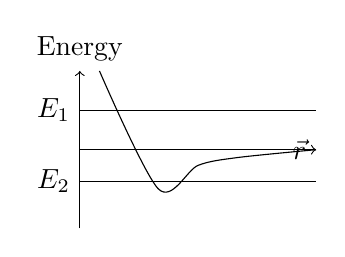
\begin{tikzpicture} \draw[->] (0,-1)--(0,1) node[anchor=south]{Energy}; \draw[->] (0,0)--(3,0) node[anchor=east]{$\vec{r}$}; \draw plot [smooth] coordinates {(0.25,1) (1,-.5) (1.5,-.2) (2,-.1) (3,0) }; \draw (0,.5)node[anchor=east]{$E_1$} --(3,.5); \draw (0,-.4)node[anchor=east]{$E_2$}--(3,-.4); \end{tikzpicture} \end{center} Between the certain energy levels, there is different behavior. $E_1$ corresponds ot a hyperbola, since ther's only one turning point, it will make one turn, which is a path that looks like \begin{center} 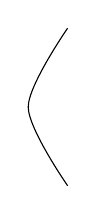
\begin{tikzpicture} \draw plot [smooth] coordinates {(.5,1) (0,0) (.5,-1)}; \end{tikzpicture} \end{center} at $E_2$, it will be an ellipse, from $r_1$ to $r_2$ (i.e. the places $E_2$ intersectes energy). At $E_4$, you should get a parabola (lowest point on the energy graph). We can also solve for $\theta(t),r(t)$ using $L,E$ are constant. In principle, we coould solve and make plots in terms of time etc, but we also want to see plots of $r(\theta$, $\theta(r)$. We can use conservation of angualr momentum to achieve this goal. $\dv{\theta}{t}=\frac{l}{mr^2}$, which gives us $ldt=mr^2d\theta$. We can write this as \begin{equation} d\theta=\frac{ldr}{mr^2\sqrt{\frac{2}{m}\left(E-V(r)-\frac{l^2}{2mr^2}\right)}} \end{equation} with potential written as inverse $r$, we get \begin{equation} \theta=\theta_0+\int_{r_0}^r\frac{dr}{r^2\sqrt{\frac{2mE}{l^2}-\frac{2mV}{l^2}-\frac{l}{r^2}}} \end{equation} making a u-sub, for $r=\frac{1}{u}$, we get \begin{align} \theta=\theta_0\int_{u_0}^u\frac{du}{\sqrt{\frac{2mE}{l^2}-\frac{2mV}{l^2}-u^2}} \end{align} To be continued thursday.
\end{document}
